\documentclass[12pt]{book}
\usepackage[utf8]{inputenc}
\usepackage[T1]{fontenc}
\usepackage{tocbibind}
\usepackage{mathptmx}
\usepackage{geometry}
\usepackage{mathtools}
\usepackage[english]{babel}
\usepackage{graphicx}
\usepackage{subcaption}
\usepackage{stackengine}
\usepackage[os=win]{menukeys}
\usepackage{hyperref}
\usepackage{xcolor}
\usepackage{color}
\usepackage{tikz}
\usepackage[yyyymmdd,hhmmss]{datetime}
\usepackage{etoolbox}
\usepackage[inline]{enumitem}
\usepackage{listings}
\usepackage{booktabs}
\usepackage[os=win]{menukeys}
\usepackage{parskip}
\usepackage{minted} % paket lingkungan kode sumber

\newcommand{\WindowsLogo}{\raisebox{-0.1em}{
\includegraphics[height=0.8em]{images/logo/Windows_3_logo_simplified}}}
%\newcommand{\PowerLogo}{\raisebox{-0.1em}{
\includegraphics[height=0.8em]{images/logo/power}}}
\newcommand{\WinKey}{\keys{\WindowsLogo}}
\newcommand{\PowerKey}{\keys{\PowerLogo}}

%%%%% Mengganti label "Contents" ke "Daftar Isi" %%%%%
\addto\captionsenglish{\renewcommand{\contentsname}{Daftar Isi}}

%%%%% Mengganti label "Chapter" ke "Bab" %%%%%
\addto\captionsenglish{\renewcommand{\chaptername}{Bab}}

%%%%% Mengganti label "Figure" ke "Gambar" %%%%%
\addto\captionsenglish{\renewcommand{\figurename}{Gambar}}

%%%%% Mengganti label "List of Figures" ke "Daftar Gambar" %%%%%
\addto\captionsenglish{\renewcommand{\listfigurename}{Daftar Gambar}}

%%%%% Mengganti label "Table" ke "Tabel" %%%%%
\addto\captionsenglish{\renewcommand{\tablename}{Tabel}}

%%%%% Mengganti label "List of Tables" ke "Daftar Table" %%%%%
\addto\captionsenglish{\renewcommand{\listtablename}{Daftar Tabel}}

\hypersetup{
	colorlinks=true, %set true if you want colored links
	linktoc=all,     %set to all if you want both sections and subsections linked
	linkcolor=blue,  %choose some color if you want links to stand out
	urlcolor=blue,   %url color
}

\geometry{
	a4paper,
	left=10mm,
	right=10mm,
	top=15mm,
	bottom=15mm,
}

\date{}

\hypersetup{citecolor=black}

\definecolor{LightGray}{gray}{0.95}

%\pagecolor[rgb]{0.1,0.1,0.1}
%\color[rgb]{1,1,1}

\lstset
{
	language=bash,
	breaklines=true,
	basicstyle=\tt\normalsize,
	frame = single
}

\begin{document}
	\frontmatter
	\begin{titlepage}
		\centering
		{\LARGE \bf Panduan Instalasi Software Open-Source untuk Pengembangan Sistem Tertanam}
		\vfill
		{\Large Achmadi ST MT}
		\vfill
		Update: {\today}
		\vfill
		
\includegraphics[width=250pt]{images/pancasila}
		\vfill
		\vfill
		\vfill
	\end{titlepage}
	
	%%%%%%%%%%%%%%%%%%%%%%%%%%%%%%%%%%%%%%%%%%%%%%%%%%%%%%%%%%%%%%%%%
	
	\newpage
	\tableofcontents
	\listoffigures
	\listoftables
	
	%%%%%%%%%%%%%%%%%%%%%%%%%%%%%%%%%%%%%%%%%%%%%%%%%%%%%%%%%%%%%%%%%
	
	%%%%%%%%%%%%%%%%%%%%%%%%%%%%%%%%%%%%%%%%%%%%%%%%%%%%%%%%%%%%%%%%%
	
	\newpage
	\chapter{Penggunaan Buku}
	
	\section{Umum}
	Buku ini dibuat dengan tujuan penggunaan utama sebagai panduan digital untuk mempermudah search dan copy-paste.
	Anda tidak perlu mencetak buku ini ke bentuk kertas.
	Seluruh navigasi buku ini diharapkan menggunakan klik ke hyperlink di Daftar Isi,
	atau menggunakan tampilan \textbf{Index} yang tersedia di \textbf{SideBar} program pembaca PDF yang anda gunakan.
	
	\section{Petunjuk}
	Beberapa petunjuk yang digunakan di buku ini:
	\begin{itemize}
		\item \textbf{Cetak Tebal}: Menginformasikan identifier (keyword, variabel, fungsi, alamat, nama file, dst) yang berada di suatu paragraf
		\item \textbf{TIPS:} Menginformasikan hal-hal yang dapat membantu atau pengetahuan tambahan.
		\item \textbf{PERINGATAN:} Menginformasikan hal-hal yang benar-benar harus diperhatikan.
		\item Bentuk \menu[,]{File,Save} dan \keys[,]{ctrl,s} menunjukkan klik menu dan tombol keyboard.
	\end{itemize}
	
	%%%%%%%%%%%%%%%%%%%%%%%%%%%%%%%%%%%%%%%%%%%%%%%%%%%%%%%%%%%%%%%%%
	
	\newpage
	\mainmatter
	\chapter{Sistem Operasi}
	
	\section{Rekomendasi Sistem Operasi}
	
	Berikut adalah sistem operasi yang direkomendasikan dengan pertimbangan:
	
	\begin{itemize}
		\item Software terbuka menyediakan untuk lingkungan sistem operasi tersebut.
		
		\item Update untuk sistem operasi tersebut cukup dekat dengan \textit{upstream}.
		
		\item Penulis menggunakan sistem operasi tersebut secara pribadi.
	\end{itemize}
	
	\subsection{Arch Linux}
	
	Arch Linux adalah sistem operasi berbasis GNU/Linux yang bersifat sederhana dan fleksibel.
	Sistem Operasi ini dibangun untuk pengguna GNU/Linux level menengah dan seterusnya.
	Untuk pemula atau tidak mampu mencoba di lingkungan virtual/emulasi, silahkan pilih opsi lain.
	
	Berikut beberapa contoh panduan instalasi:
	
	\begin{itemize}
		\item Instalasi Arch Linux: \url{https://itsfoss.com/install-arch-linux/}.
		
		\item Instalasi Desktop (contoh Mate Desktop): \\
		\url{https://www.tecmint.com/install-mate-desktop-in-arch-linux/}
	\end{itemize}
	
	\begin{figure}[!ht]
		\centering
		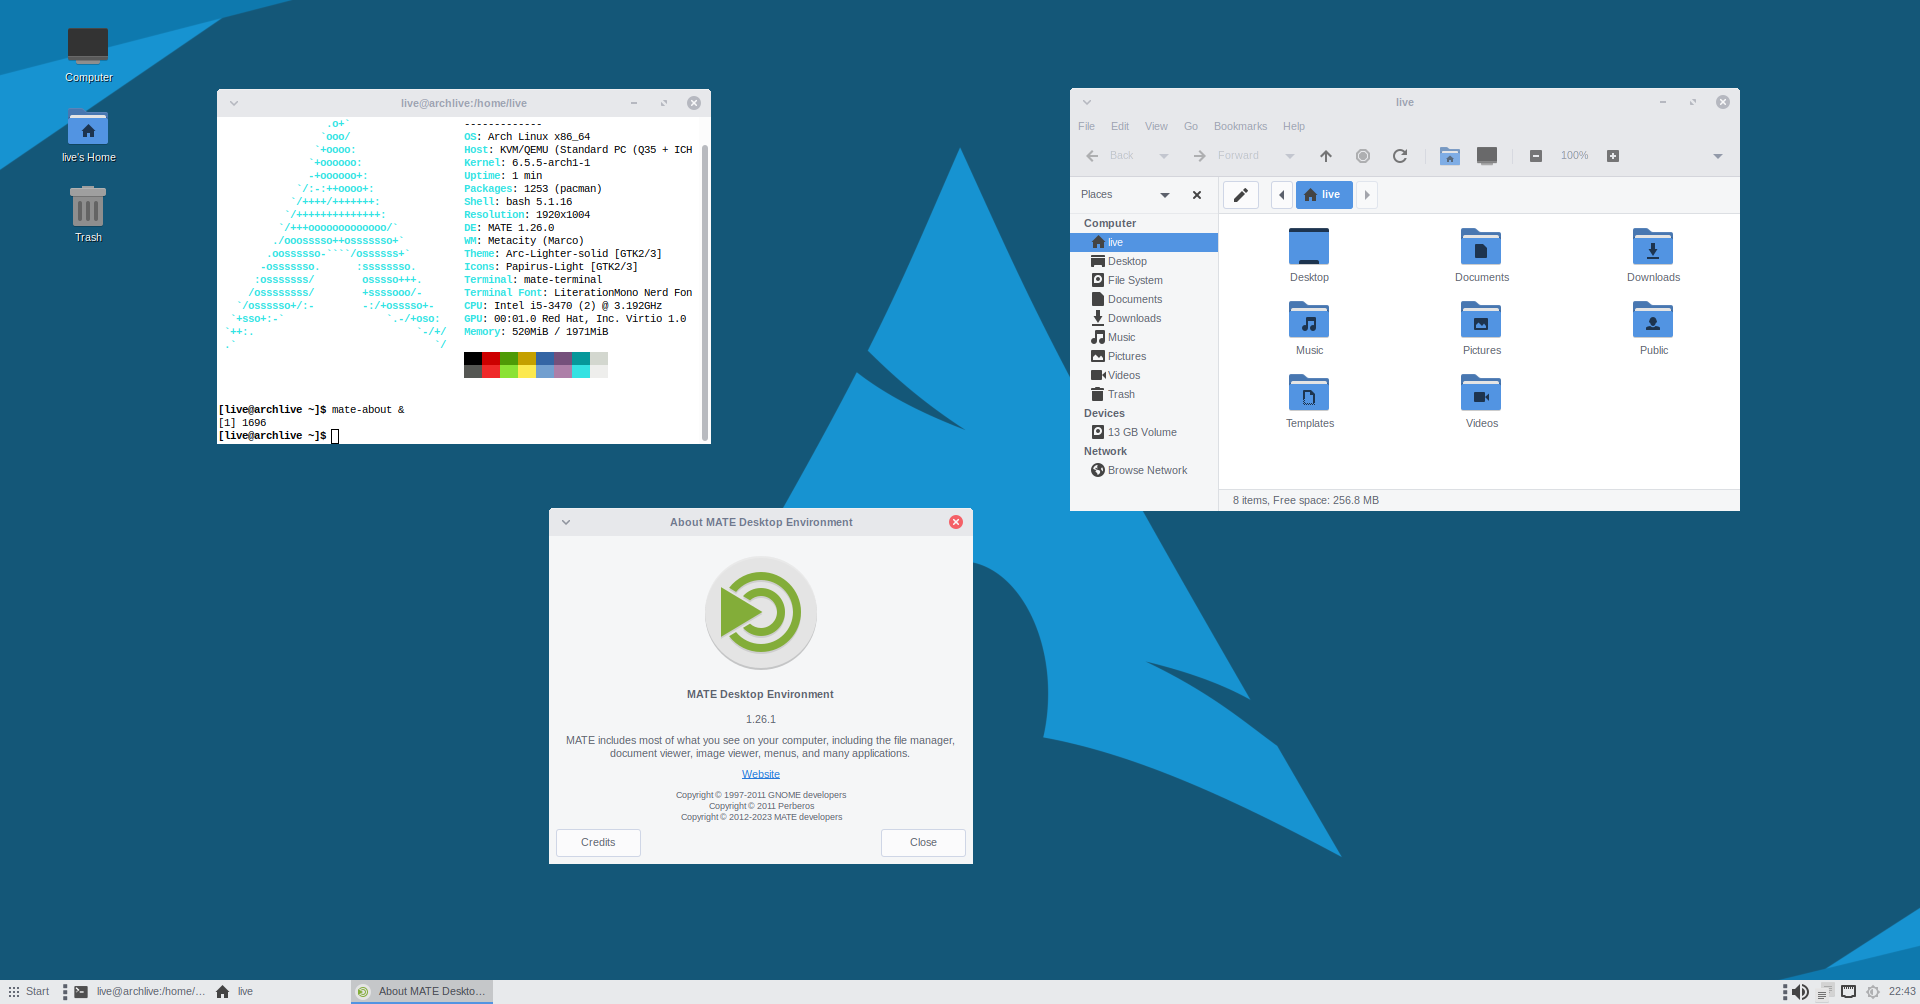
\includegraphics[width=0.8\textwidth]{images/os/archmate}
		\caption{Contoh Arch Linux}
	\end{figure}
	
	\newpage
	\subsection{Manjaro}
	
	Manjaro adalah sistem operasi turunan Arch Linux yang menyediakan image ISO yang siap install secara offline.
	Manjaro cenderung lebih ramah untuk pengguna pemula.
	
	Berikut contoh instalasi:
	
	\begin{itemize}
		\item Situs Manjaro: \url{https://manjaro.org/}
		
		\item Download ISO untuk Mate Desktop Minimal sebagai contoh: \\
		\url{https://download.manjaro.org/mate/23.0.1/manjaro-mate-23.0.1-minimal-230921-linux65.iso}
		
		\item Instalasi Manjaro: \\
		\url{https://itsfoss.com/install-manjaro-linux/}
	\end{itemize}
	
	\begin{figure}[!ht]
		\centering
		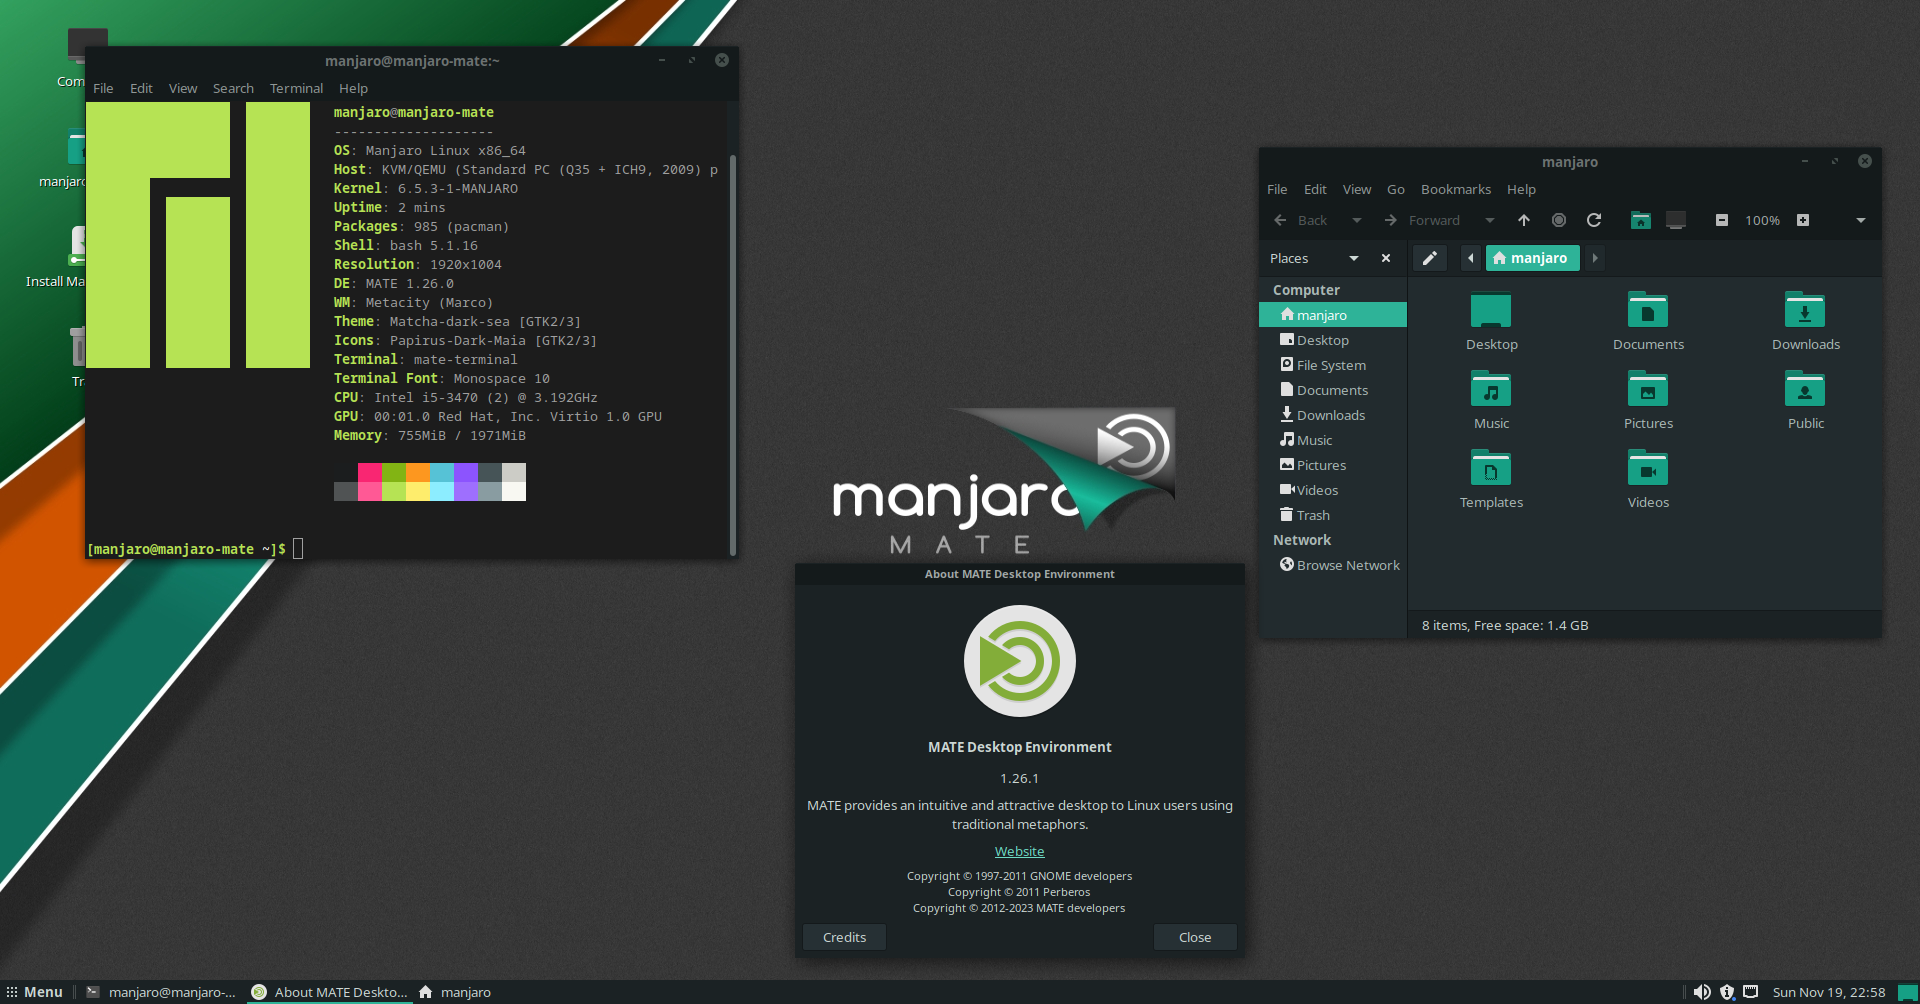
\includegraphics[width=0.8\textwidth]{images/os/manjaro}
		\caption{Contoh Manjaro}
	\end{figure}
	
	Selanjutnya, update instalasi secara online dengan perintah di terminal (\menu[,]{Menu,System Tools,Mate Terminal}):
	
	\begin{minted}[frame=lines,framesep=2mm,fontsize=\normalsize,bgcolor=LightGray]{sh}
sudo pacman -Syu
	\end{minted}
	
	\subsection{Windows MSYS2}
	
	MSYS2 adalah software distribusi yang menyediakan lingkungan GNU ke sistem operasi Windows.
	MSYS2 merupakan pengganti dari proyek Cygwin dan menggunakan Pacman sebagai pengelola paket layaknya Arch-Linux.
	
	\textbf{PERINGATAN:} MSYS2 versi terbaru membutuhkan Windows 8.1 atau lebih tinggi di 64-bit.
	
	Berikut contoh instalasi:
	
	\begin{itemize}
		\item Situs MSYS2: \url{https://www.msys2.org/}
		
		\item Download Installer: \url{https://github.com/msys2/msys2-installer/releases/download/2023-10-26/msys2-x86_64-20231026.exe}
		
	\end{itemize}
	
	Direkomendasikan menggunakan \textbf{MSYS2 MINGW64} sebagai profil utama.
	
	\newpage
	\begin{figure}[!ht]
		\centering
		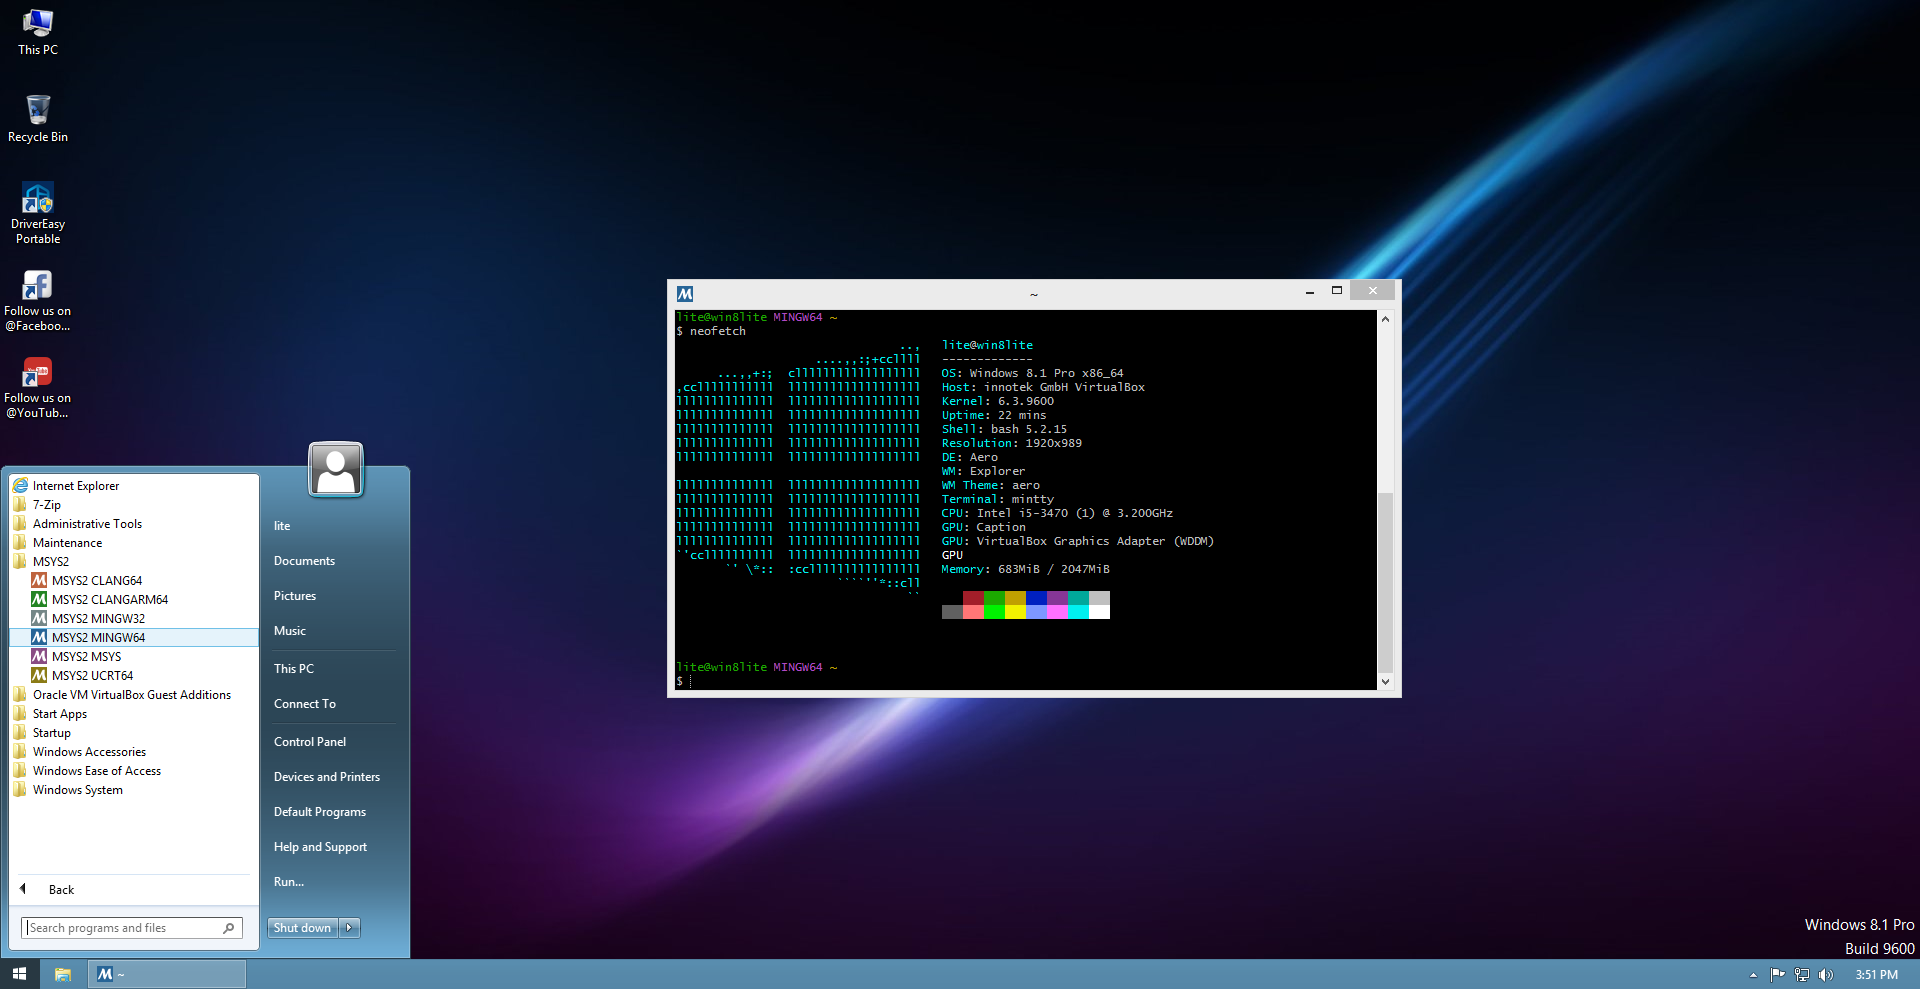
\includegraphics[width=0.8\textwidth]{images/os/msys2}
		\caption{Contoh MSYS2 di Windows 8.1}
	\end{figure}
	
	\section{Alternatif Sistem Operasi}
	
	Sebagai alternatif, dapat pula digunakan sistem operasi berikut ini.
	
	\subsection{Windows tanpa MSYS2}
	
	Windows 8.1, Windows 10, dan Windows 11 dapat digunakan sebagai sistem operasi dengan proses instalasi software sebagaimana umumnya.
	
	\textbf{TIPS:} KiCAD, Electron, dan banyak software tidak lagi mendukung Windows 7 dan sebelumnya.
	
	\begin{figure}[!ht]
		\centering
		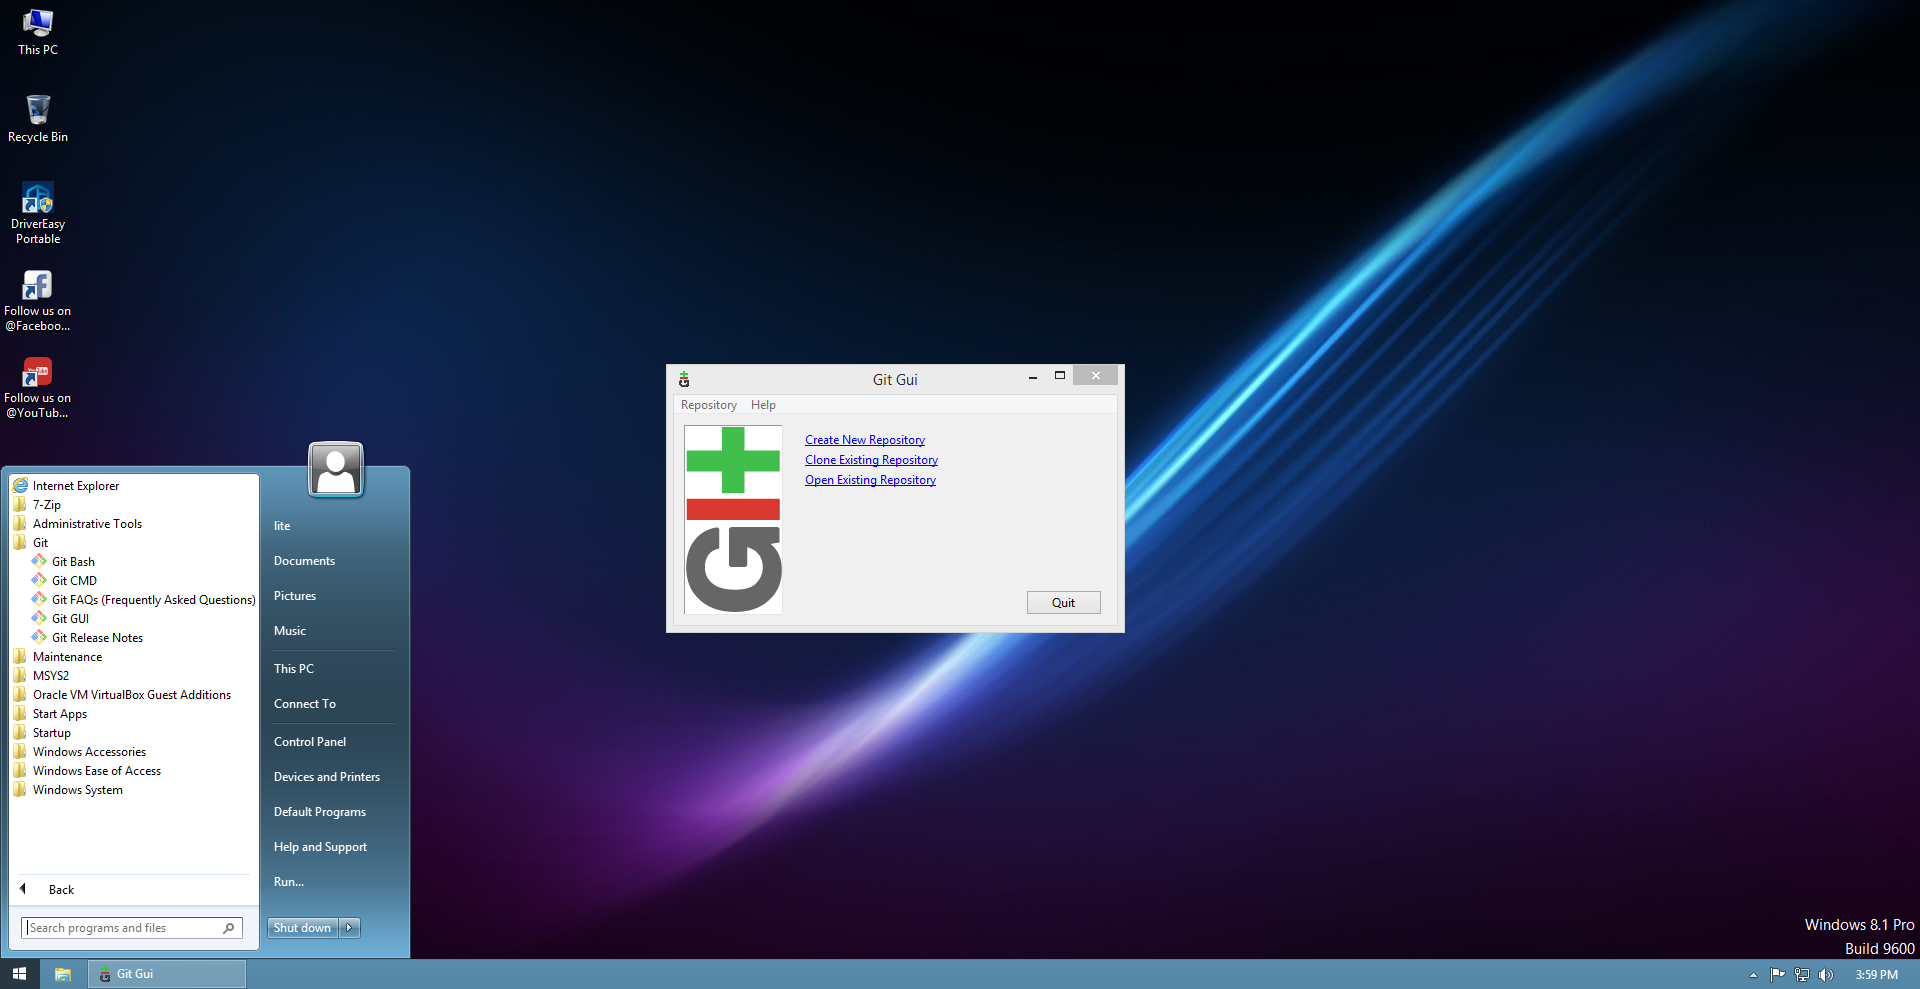
\includegraphics[width=0.8\textwidth]{images/os/windows}
		\caption{Contoh Windows 8.1}
	\end{figure}
	
	\subsection{Debian dan turunannya}
	
	Selain Arch-Linux dan turunannya seperti Manjaro, dapat pula digunakan sistem operasi Debian dan turunannya seperti Ubuntu atau Linux-Mint.
	Untuk panduan dalam buku ini, tidak dicantumkan instalasi menggunakan Debian atau Ubuntu.
	
	%%%%%%%%%%%%%%%%%%%%%%%%%%%%%%%%%%%%%%%%%%%%%%%%%%%%%%%%%%%%%%%%%
	
	\newpage
	\chapter{Git}
	
	\section{Ringkasan}
	
	Git adalah software yang membantu programmer untuk cek perubahan berkas teks (dikenal sebagai \textit{patch})
	dan menyimpannya sebagai versi pengembangan (dikenal sebagai \textit{commit}).
	
	Penjelasan tentang Git dapat dilihat di laman utama: \url{https://git-scm.com/}.
	
	\section{Instalasi}
	
	Berikut panduan ringkas untuk instalasi:
	
	\subsection{Arch-Linux atau Manjaro}
	
	Instalasi secara online melalui perintah terminal:

	\begin{minted}[frame=lines,framesep=2mm,fontsize=\normalsize,bgcolor=LightGray]{sh}
sudo pacman -S git tig
	\end{minted}
	
	kemudian dapat dicek dengan perintah:
	
	\begin{minted}[frame=lines,framesep=2mm,fontsize=\normalsize,bgcolor=LightGray]{sh}
git --version
	\end{minted}
	
	\begin{figure}[!ht]
		\centering
		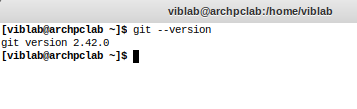
\includegraphics[width=0.7\textwidth]{images/git/gitvergnu}
		\caption{Git Version GNU/Linux}
	\end{figure}
	
	\subsection{MSYS2}
	
	Instalasi secara online melalui perintah terminal:
	
	\begin{minted}[frame=lines,framesep=2mm,fontsize=\normalsize,bgcolor=LightGray]{sh}
pacman -S git tig
	\end{minted}
	
	kemudian dapat dicek dengan perintah:
	
	\begin{minted}[frame=lines,framesep=2mm,fontsize=\normalsize,bgcolor=LightGray]{sh}
git --version
	\end{minted}
	
	\begin{figure}[!ht]
		\centering
		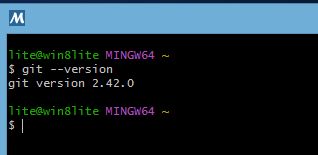
\includegraphics[width=0.5\textwidth]{images/git/gitvermsys}
		\caption{Git Version MSYS2}
	\end{figure}
	
	\subsection{Windows}
	
	Download non-portable installer di laman: \url{https://git-scm.com/download/win}.
	
	Install sebagaimana software pada umumnya:
	
	\begin{figure}[!ht]
		\centering
		\begin{subfigure}[t]{0.5\textwidth}
			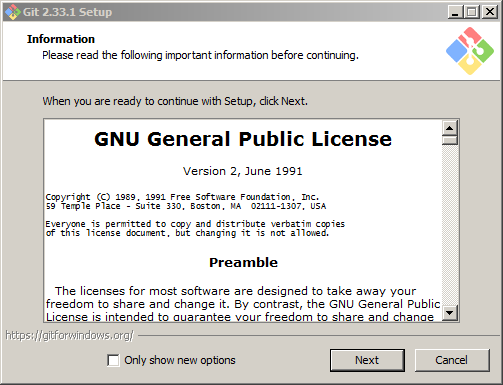
\includegraphics[width=\textwidth]{images/git/gitwininstall}
			\caption{Install Git}
		\end{subfigure}
		\begin{subfigure}[t]{0.3\textwidth}
			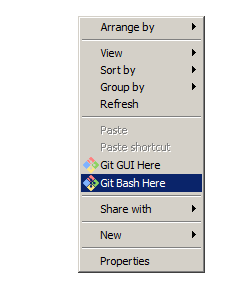
\includegraphics[width=\textwidth]{images/git/gitwinmenu}
			\caption{Akses Git Bash}
		\end{subfigure}
		\caption{Git Windows}
	\end{figure}
	
	\newpage
	kemudian dapat dicek dengan perintah:
	
	\begin{minted}[frame=lines,framesep=2mm,fontsize=\normalsize,bgcolor=LightGray]{sh}
git --version
	\end{minted}
	
	\begin{figure}[!ht]
		\centering
		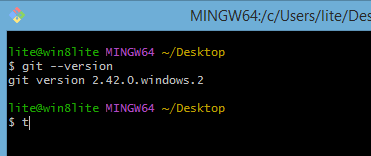
\includegraphics[width=0.5\textwidth]{images/git/gitverwin}
		\caption{Git Version Windows}
	\end{figure}
	
	\section{Konfigurasi}
	
	Konfigurasi umum untuk git dapat dilakukan melalui terminal (atau terminal MSYS2 atau Git-Bash).
	Sebagai contoh:
	
	\begin{minted}[frame=lines,framesep=2mm,fontsize=\normalsize,bgcolor=LightGray]{sh}
git config --global init.defaultBranch main
git config --global user.name "mekatronik-achmadi"
git config --global user.email "mekatronik.achmadi@gmail.com"
	\end{minted}
	
	Berkas konfigurasi dapat dicek di alamat:
	
	\begin{itemize}
		\item Arch-Linux/Manjaro: \textbf{/home/username/.gitconfig}
		
		\item MSYS2: \textbf{C:\textbackslash msys64\textbackslash home\textbackslash username\textbackslash .gitconfig}
		
		\item Git: \textbf{C:\textbackslash Users\textbackslash username\textbackslash .gitconfig}
	\end{itemize}
	
	Contoh isi konfigurasi:
	
	\begin{figure}[!ht]
		\centering
		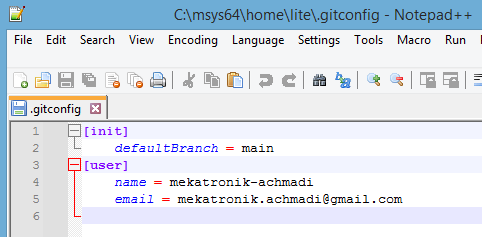
\includegraphics[width=0.6\textwidth]{images/git/gitconfig}
		\caption{Konfigurasi Git}
	\end{figure}
	
	\newpage
	\section{GUI}
	
	Git menyediakan GUI yang dapat diakses dengan menu perintah terminal:
	
	\begin{minted}[frame=lines,framesep=2mm,fontsize=\normalsize,bgcolor=LightGray]{sh}
git gui
	\end{minted}
	
	\begin{figure}[!ht]
		\centering
		\begin{subfigure}[t]{0.45\textwidth}
			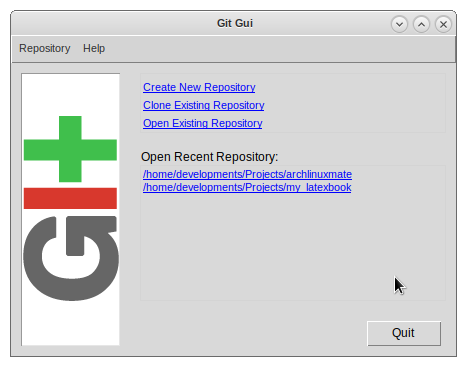
\includegraphics[width=\textwidth]{images/git/gitgui}
			\caption{Start}
		\end{subfigure}
		\begin{subfigure}[t]{0.45\textwidth}
			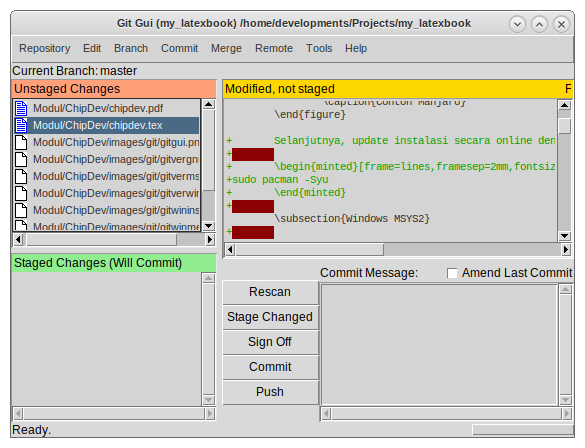
\includegraphics[width=\textwidth]{images/git/gitstage}
			\caption{Staging}
		\end{subfigure}
		\caption{Git GUI}
	\end{figure}
	
	\section{Commit Log}
	
	Commit log dapat dicek melalui perintah \textbf{tig} atau melalui GUI di menu \menu[,]{Repository, Visualize History}
	
	\begin{figure}[!ht]
		\centering
		\begin{subfigure}[t]{0.45\textwidth}
			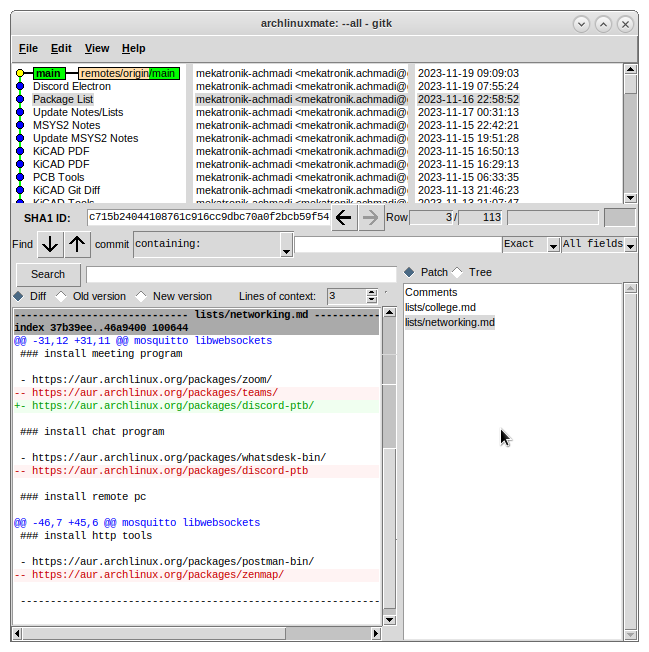
\includegraphics[width=\textwidth]{images/git/gitk}
			\caption{Gitk}
		\end{subfigure}
		\begin{subfigure}[t]{0.45\textwidth}
			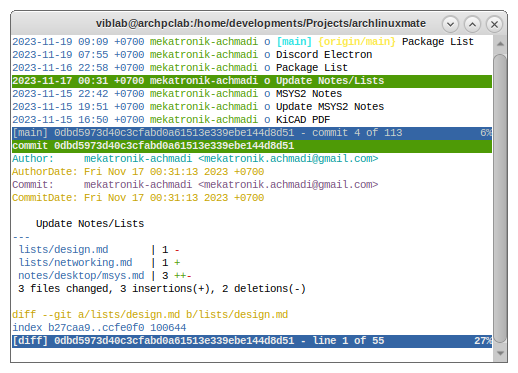
\includegraphics[width=\textwidth]{images/git/tig}
			\caption{Tig}
		\end{subfigure}
		\caption{Git Commit Log}
	\end{figure}
	
	\newpage
	\section{Remote Git}
	
	Remote Git adalah layanan server yang dapat digunakan sebagai salinan git di komputer lokal.
	Remote sangat bermanfaat untuk cadangan maupun alir kerja kolaborasi seperti git-push dan git-pull.
	
	\subsection{Workflow}
	
	Secara umum, berikut workflow git dan remote yang dapat dilakukan berulang:
	
	\begin{figure}[!ht]
		\centering
		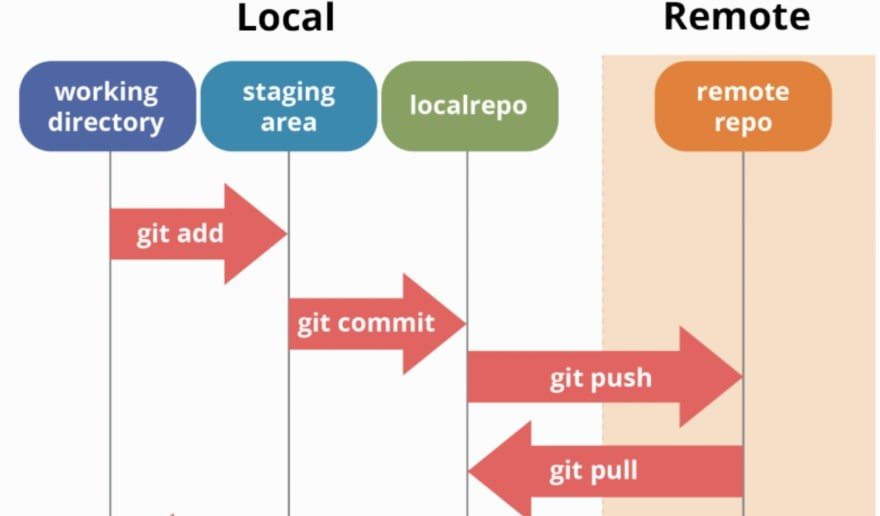
\includegraphics[width=0.8\textwidth]{images/git/githubworkflow}
		\caption{Workflow}
	\end{figure}
	
	\subsection{Git-Web}
	
	Git Web adalah server remote yang tersedia satu paket dengan software git.
	Git Web bekerja sama dengan webserver seperti Apache atau Lighthttpd.
	
	\begin{figure}[!ht]
		\centering
		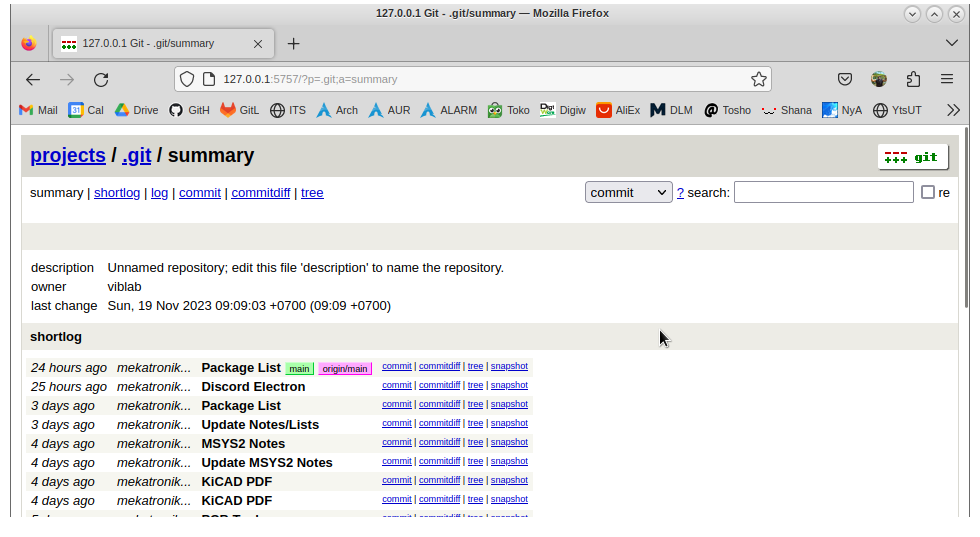
\includegraphics[width=0.75\textwidth]{images/git/gitweb}
		\caption{Git Web}
	\end{figure}
	
	\subsection{Github}
	
	Github adalah proprietary remote git berbasis cloud yang dibangun oleh Github, Inc yang kini telah dibeli oleh Microsoft.
	Github ditulis dalam Ruby dan Javascript.
	Laman Github: \url{https://github.com/}.
	
	\begin{figure}[!ht]
		\centering
		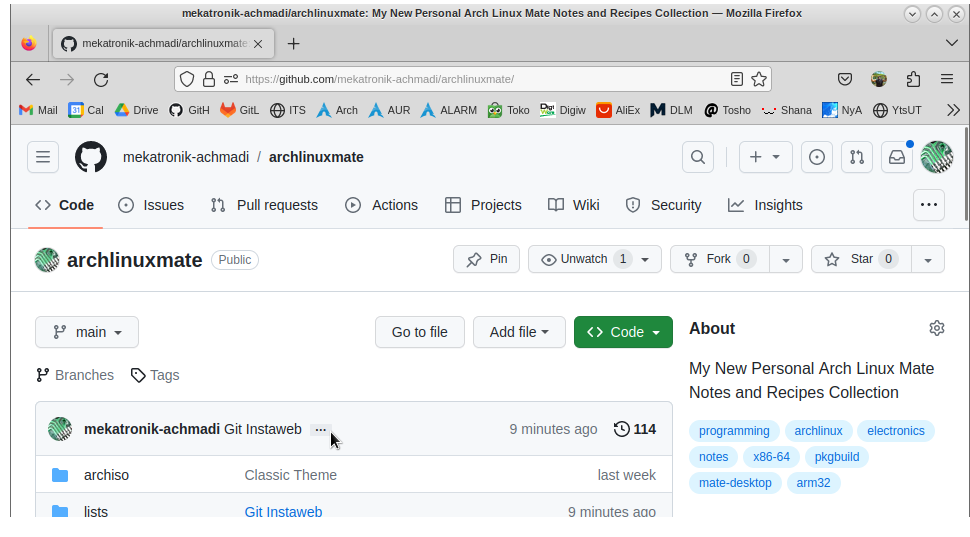
\includegraphics[width=0.65\textwidth]{images/git/github}
		\caption{Contoh Github}
	\end{figure}
	
	\textbf{TIPS:} Untuk melakukan push di Github repository, pastikan memiliki token yang valid.
	
	\subsection{Gitlab}
	
	Gitlab adalah remote git bersifat open-soure yang dibangun oleh Gitlab, Inc.
	Gitlab ditulis dalam Ruby dan Javascript.
	Laman Gitlab: \url{https://gitlab.com/}.
	
	\begin{figure}[!ht]
		\centering
		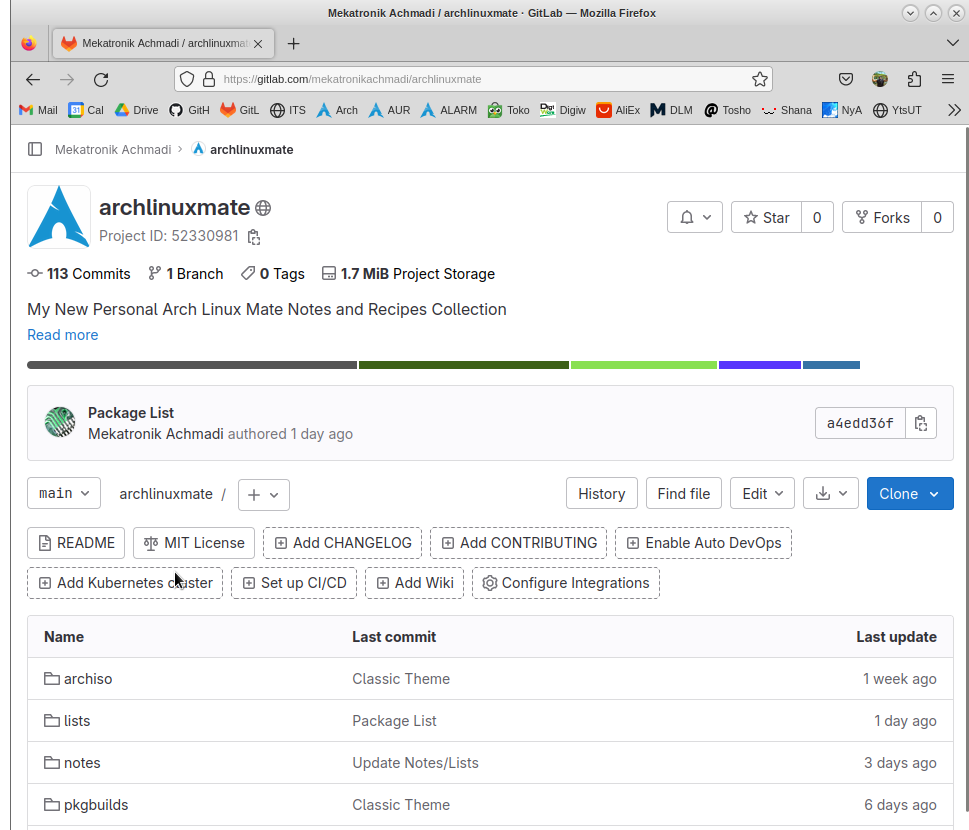
\includegraphics[width=0.65\textwidth]{images/git/gitlab}
		\caption{Contoh Gitlab}
	\end{figure}
	
	\textbf{TIPS:} Gitlab juga menyediakan paket \textit{core-server} yang dapat diinstall di komputer anda layaknya GitWeb.
	
	%%%%%%%%%%%%%%%%%%%%%%%%%%%%%%%%%%%%%%%%%%%%%%%%%%%%%%%%%%%%%%%%%
	
	\newpage
	\chapter{KiCAD}
	
	\section{Ringkasan}
	
	KiCAD adalah paket software EDA (Electronic Design Automation) yang dikembangkan untuk perancangan papan sirkuit elektronik tercetak (Printed Circuit Board atau PCB)
	secara professional yang bersifat gratis dan terbuka.
	
	KiCAD dapat disandingkan dengan perangkat perancangan PCB professional lain seperti Altium, Diptrace, EasyEDA, dan lainnya.
	KiCAD tersedia untuk sistem operasi Windows dan GNU/Linux.
	
	Berikut adalah tampilan 4 software utama dalam paket software KiCAD:
	\begin{figure}[!ht]
		\centering
		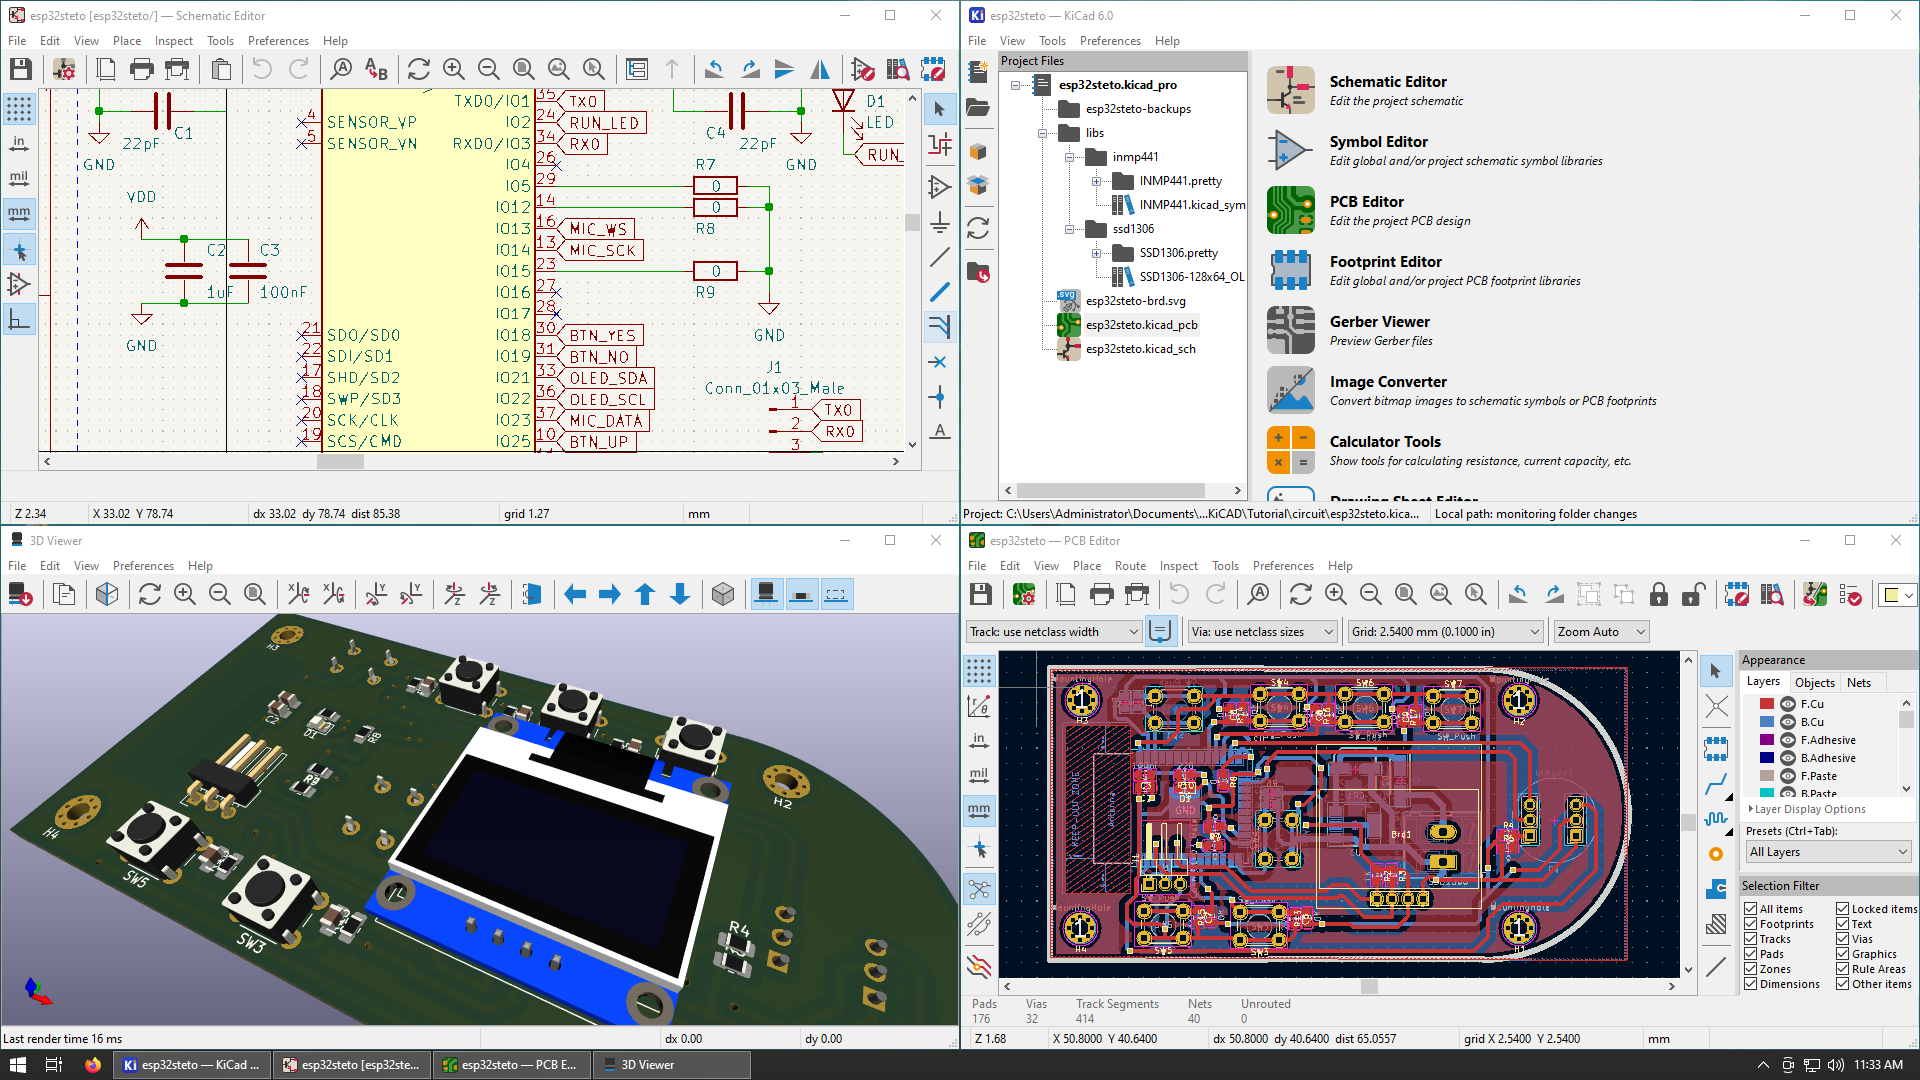
\includegraphics[width=\textwidth]{images/kicad/kicad_windows10}
		\caption{Tampilan KiCAD Windows 10}
	\end{figure}
	
	\textbf{PERINGATAN:} Instalasi lengkap KiCAD menghabiskan ruang kisaran 6.5GB dengan 5G adalah model 3D komponen.
	
	\newpage
	\section{Instalasi}
	
	Berikut panduan ringkas untuk instalasi:
	
	\subsection{Arch-Linux atau Manjaro}
	
	Instalasi secara online melalui perintah terminal:
	
	\begin{minted}[frame=lines,framesep=2mm,fontsize=\normalsize,bgcolor=LightGray]{sh}
sudo pacman -S kicad kicad-library kicad-library-3d
	\end{minted}
	
	KiCAD dapat dijalankan dari menu \menu[,]{Menu,Other,KiCAD} atau \menu[,]{Menu,Programming,KiCAD}
	
	\begin{figure}[!ht]
		\centering
		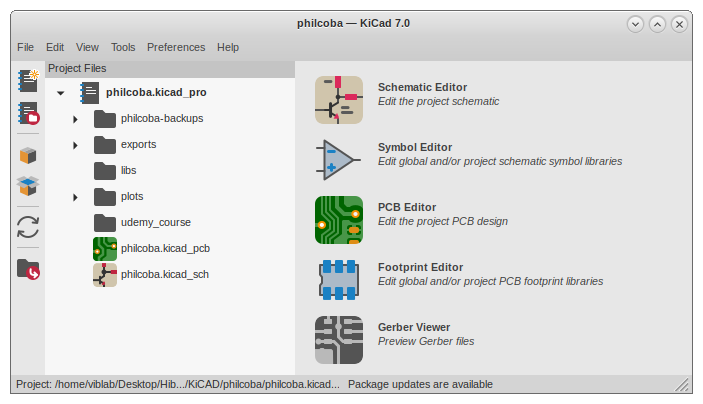
\includegraphics[width=0.55\textwidth]{images/kicad/kicadgnu}
		\caption{Tampilan KiCAD GNU/Linux}
	\end{figure}
	
	\subsection{MSYS2}
	
	Instalasi secara online melalui perintah terminal:
	
	\begin{minted}[frame=lines,framesep=2mm,fontsize=\normalsize,bgcolor=LightGray]{sh}
pacman -S mingw-w64-x86_64-kicad-meta
	\end{minted}
	
	Kemudian dapat dijalan melalui terminal MSYS2 dengan perintah:
	
	\begin{minted}[frame=lines,framesep=2mm,fontsize=\normalsize,bgcolor=LightGray]{sh}
kicad
	\end{minted}
	
	\begin{figure}[!ht]
		\centering
		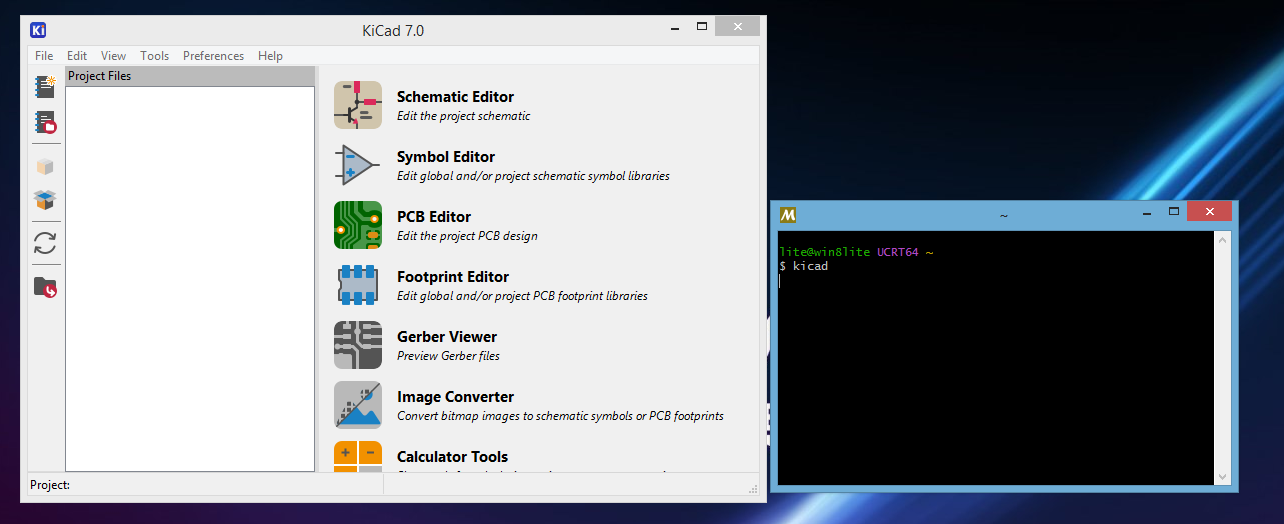
\includegraphics[width=0.55\textwidth]{images/kicad/kicadmsys2}
		\caption{Tampilan KiCAD MSYS2}
	\end{figure}
	
	\subsection{Windows}
	
	Untuk Windows tanpa MSYS2, installer dapat didownload di halaman: \url{https://www.kicad.org/download/windows/}.
	Atau di halaman rilis Github: \url{https://github.com/KiCad/kicad-source-mirror/releases}.
	
	\begin{figure}[!ht]
		\centering
		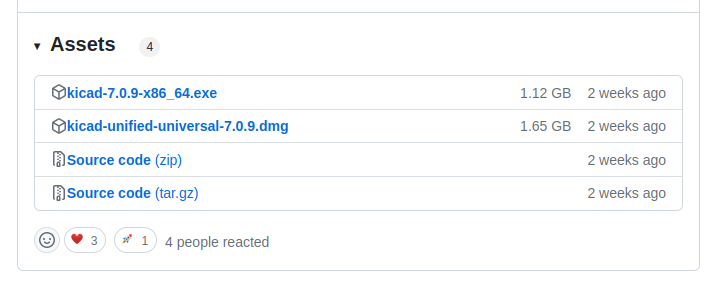
\includegraphics[width=0.7\textwidth]{images/kicad/kicadgithub}
		\caption{Github KiCAD}
	\end{figure}
	
	Instal sebagaimana umumnya. Model 3D dapat tidak diinstal untuk menghemat ruang.
	
	\begin{figure}[!ht]
		\centering
		\begin{subfigure}[t]{0.45\textwidth}
			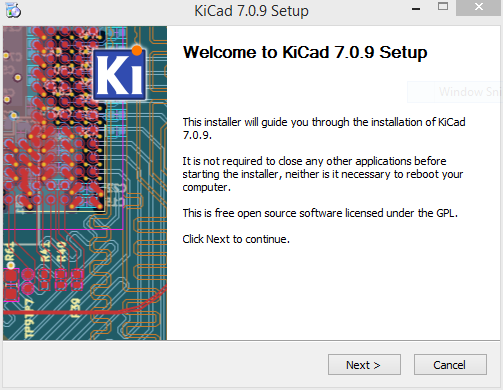
\includegraphics[width=\textwidth]{images/kicad/kicadwin0}
			\caption{Mulai Install}
		\end{subfigure}
		\begin{subfigure}[t]{0.45\textwidth}
			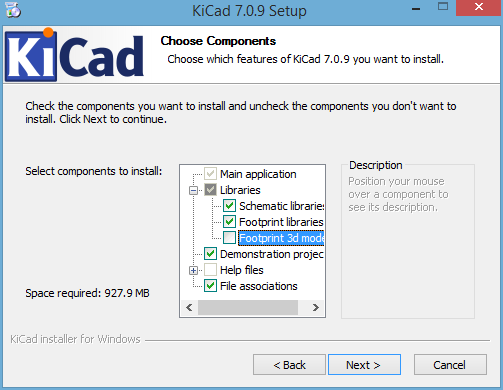
\includegraphics[width=\textwidth]{images/kicad/kicadwin1}
			\caption{Pilih Install}
		\end{subfigure}
		\caption{Install KiCAD}
	\end{figure}
	
	\begin{figure}[!ht]
		\centering
		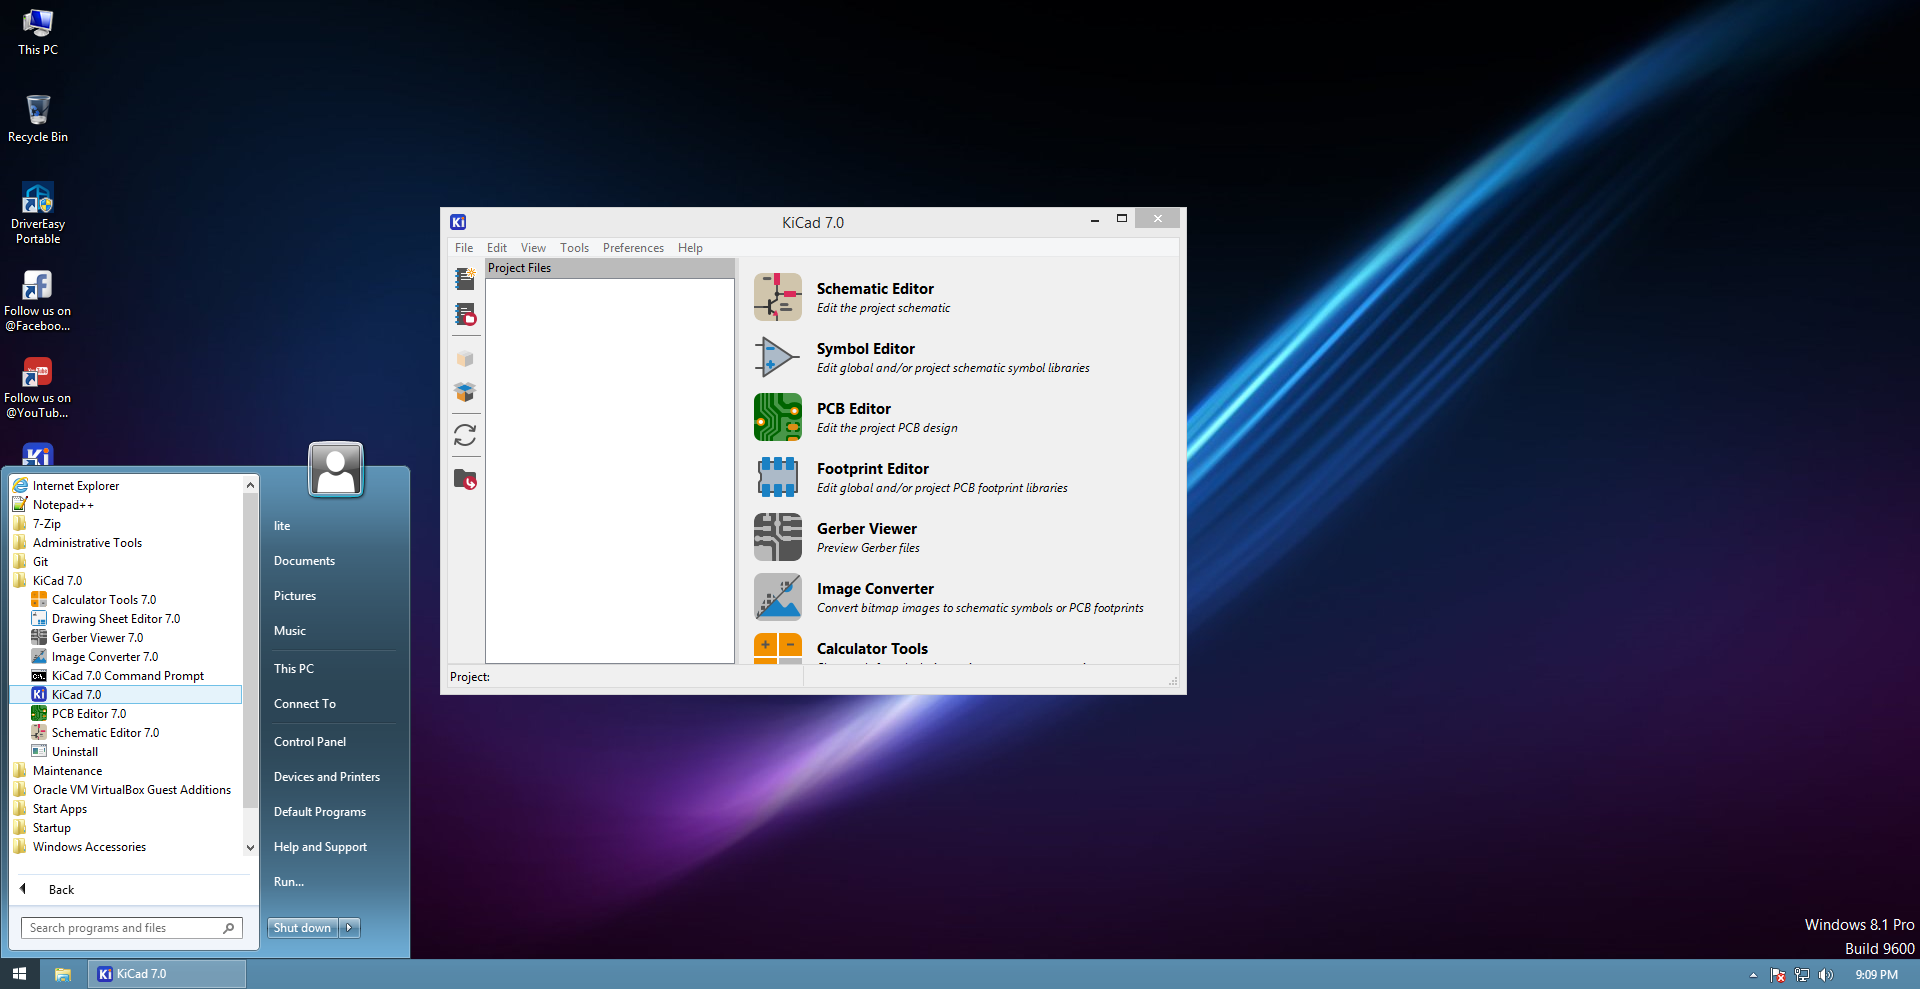
\includegraphics[width=0.7\textwidth]{images/kicad/kicadwin2}
		\caption{KiCAD Windows}
	\end{figure}
	
	\section{Addons}
	
	Untuk Install Addon, install melalui \menu[,]{Tools,Plugin and Content Manager}
	
	\begin{figure}[!ht]
		\centering
		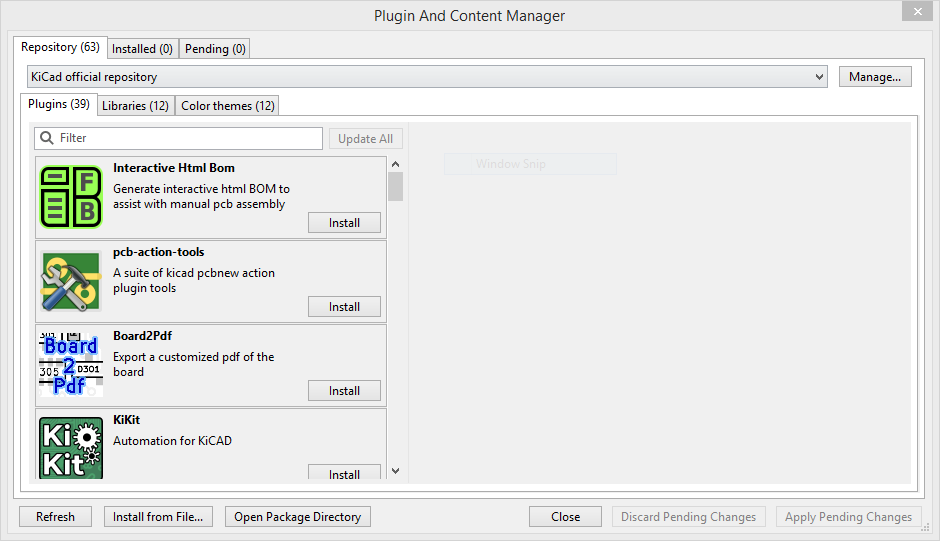
\includegraphics[width=0.7\textwidth]{images/kicad/kicadpcm}
		\caption{KiCAD Plugin Manager}
	\end{figure}
	
	Beberapa addons yang direkomendasikan:
	
	\begin{itemize}
		\item Interactive HTML BoM: \url{https://github.com/openscopeproject/InteractiveHtmlBom/}
		\item KiBuzzard: \url{https://github.com/gregdavill/KiBuzzard/}
		\item Import Lib: \url{https://github.com/Steffen-W/Import-LIB-KiCad-Plugin/}
		\item Board-PDF: \url{https://gitlab.com/dennevi/Board2Pdf/}
	\end{itemize}
	
	Beberapa Addons untuk JLC PCB:
	
	\begin{itemize}
		\item \url{https://github.com/bennymeg/JLC-Plugin-for-KiCad/}
		\item \url{https://github.com/Bouni/kicad-jlcpcb-tools/}
	\end{itemize}
	
	\section{KiCAD Git}
	
	KiCAD menyimpan berkas dalam bentuk text terformat, sehingga dapat di-\textit{track} menggunakan pengelola versi seperti Git.
	Namun \textit{patch} Git tetap menampilkan berupa text ASCII, bukan render PCB.
	
	Beberapa pola berkas yg dapat ditambahkan ke \textbf{.gitignore}:
	
	\begin{minted}[frame=lines,framesep=2mm,fontsize=\normalsize,bgcolor=LightGray]{sh}
*.lck
*-backups
*auto_saved_files#
fp-info-cache
	\end{minted}
	
	\newpage
	\section{Gerber Viewer}
	
	Gerber Viewer digunakan untuk cek berkas gerber sebelum diserahkan ke pihak fabrikasi PCB.
	
	Gerber Offline yg direkomendasikan:
	\begin{itemize}
		\item KiCAD Gerber Viewer. Tersedia satu paket dengan KiCAD.
		\item gEDA Gerbv. Ringan dan cukup sebagai gerber viewer untuk format RS-274X.\\
		\url{https://gerbv.github.io/}
	\end{itemize}
	
	\begin{figure}[!ht]
		\centering
		\begin{subfigure}[t]{0.45\textwidth}
			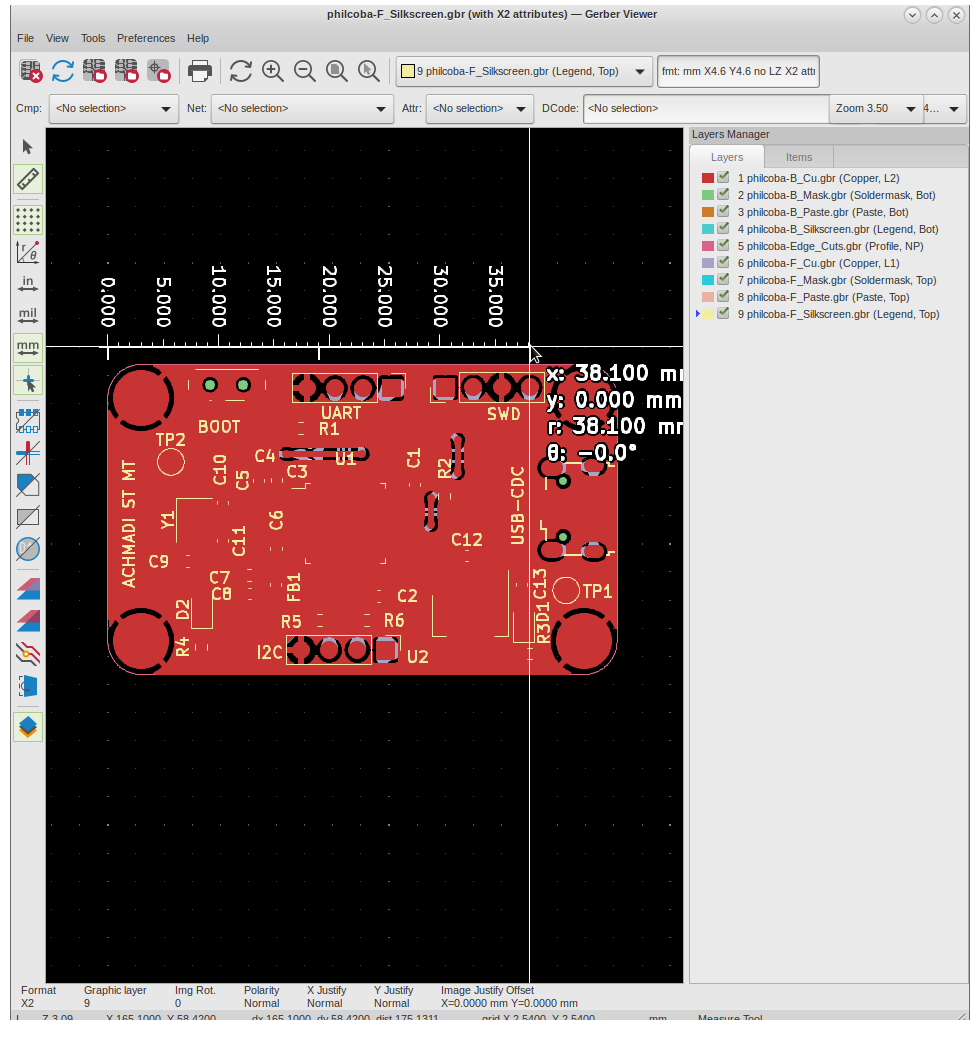
\includegraphics[width=\textwidth]{images/kicad/gerbkicad}
			\caption{KiCAD Gerber}
		\end{subfigure}
		\begin{subfigure}[t]{0.45\textwidth}
			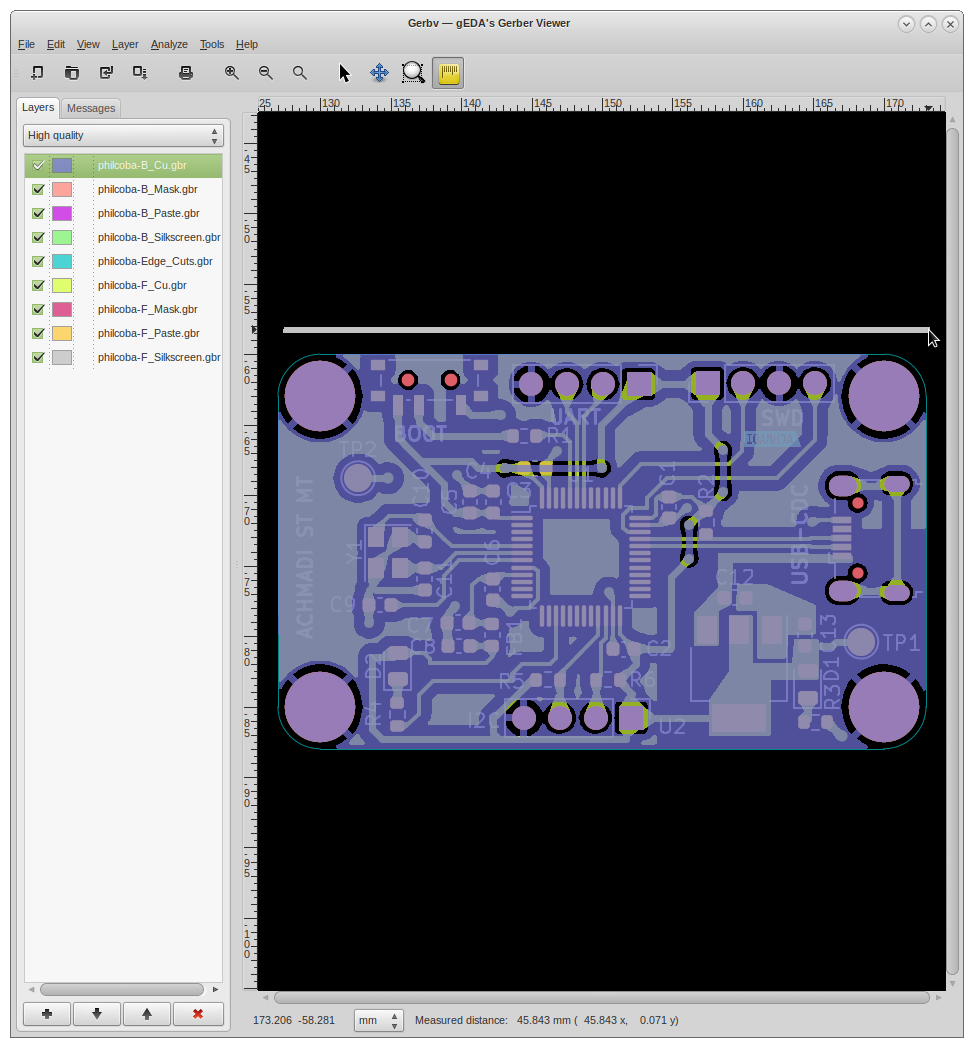
\includegraphics[width=\textwidth]{images/kicad/gerbv}
			\caption{GerbV}
		\end{subfigure}
		\caption{Gerber Viewer}
	\end{figure}
	
	Beberapa Gerber Viewer Online/Server yang dapat digunakan:
	
	\begin{itemize}
		\item Tracespace. \url{https://github.com/tracespace/tracespace}
		\item Gerai Cerdas. \url{http://www.pcbviewer.cloudcerdas.com/}
		\item PCBWay. \url{https://www.pcbway.com/project/OnlineGerberViewer.html}
		\item Elecrow. \url{https://www.elecrow.com/gerberviewer.html}
		\item PCBGogo. \url{https://www.pcbgogo.com/GerberViewer.html}
		\item GerbLook. \url{https://gerblook.org/}
		\item JLCPCB Quotes. \url{https://jlcpcb.com/RGE}
	\end{itemize}
	
	\newpage
	\begin{figure}[!ht]
		\centering
		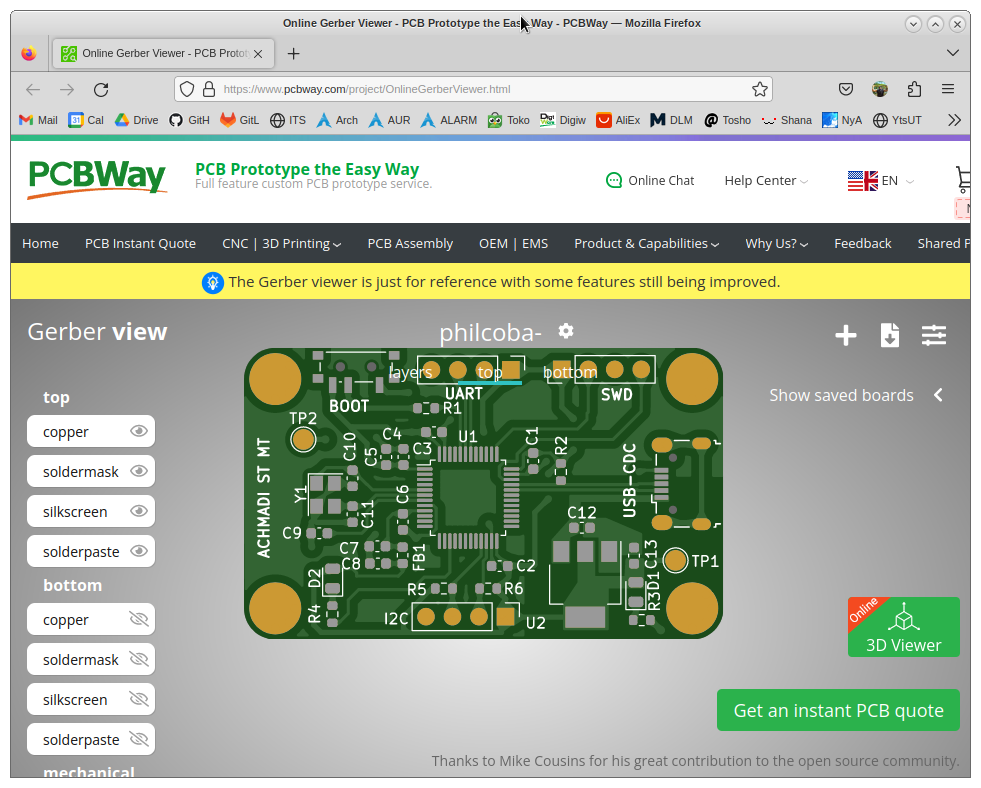
\includegraphics[width=0.7\textwidth]{images/kicad/gerbvonline}
		\caption{Online Gerber Viewer}
	\end{figure}
	
	\section{Tutorial}
	
	Berikut PDF Tutorial penggunaan KiCAD Dasar yang dapat diunduh gratis: \\
	\url{https://drive.google.com/file/d/1MCIVBWtsZTRt3-c9JOJCKUUE-283L9ly/view?usp=drive_link}
	
	%%%%%%%%%%%%%%%%%%%%%%%%%%%%%%%%%%%%%%%%%%%%%%%%%%%%%%%%%%%%%%%%%
	
	\newpage
	\chapter{ChibiOS/RT STM32}
	
	\section{Ringkasan}
	
	ChibiOS/RT adalah pustaka hardware abstraksi dan sistem operasi real-time untuk banyak chip ARM-Cortex M.
	Disini akan digunakan ARM-none-EABI GCC sebagai kompiler.
	
	Laman ChibiOS/RT: \url{https://www.chibios.org/dokuwiki/doku.php}
	
	\section{Instalasi Compiler}
	
	Berikut Instalasi compiler ARM-GCC
	
	\subsection{Arch-Linux/Manjaro}

	\begin{minted}[frame=lines,framesep=2mm,fontsize=\normalsize,bgcolor=LightGray]{sh}
sudo pacman -S base-devel arm-none-eabi-gcc arm-none-eabi-gdb arm-none-eabi-newlib
	\end{minted}
	
	instalasi dapat dicek dengan perintah
	\begin{minted}[frame=lines,framesep=2mm,fontsize=\normalsize,bgcolor=LightGray]{sh}
arm-none-eabi-gcc --version
	\end{minted}
	
	\subsection{MSYS2}
	
	\begin{minted}[frame=lines,framesep=2mm,fontsize=\normalsize,bgcolor=LightGray]{sh}
pacman -S base-devel mingw-w64-x86_64-arm-none-eabi-gcc \
mingw-w64-x86_64arm-none-eabi-gdb \
mingw-w64-x86_64arm-none-eabi-newlib
	\end{minted}
	
	instalasi dapat dicek dengan perintah
	\begin{minted}[frame=lines,framesep=2mm,fontsize=\normalsize,bgcolor=LightGray]{sh}
arm-none-eabi-gcc --version
	\end{minted}
	
	\subsection{Windows}
	
	Download 32bit installer disini: \url{https://developer.arm.com/downloads/-/gnu-rm}
	
	Install seperti pada umumnya dan tambahkan alamat \textbf{C:\textbackslash gcc-arm-suite\textbackslash bin} ke \textbf{Path} di \textbf{Environment Variables}.
	
	\section{Instalasi Driver}
	
	Beberapa Driver yang perlu diinstal jika diperlukan antara lain:
	
	\begin{itemize}
		\item Serial TTL-USB:
		\begin{itemize}
			\item CH34x: \url{https://cdn.sparkfun.com/assets/learn_tutorials/8/4/4/CH341SER.EXE}
			\item FT232RL: \url{https://ftdichip.com/drivers/vcp-drivers/}
			\item PL2303: \url{https://www.prolific.com.tw/US/ShowProduct.aspx?p_id=225&pcid=41}
			\textbf{TIPS:} Driver PL2303 mungkin akan tampil Phased-Out untuk Windows 10 dan Windows 11.
			Alternative download versi lama: \href{https://drive.google.com/file/d/11ivvhc-s3gQD2uzF0HDYm6e5w_w103FT/view}{G-Drive}
		\end{itemize}
		
		\item STM32-VCP: \url{https://www.st.com/en/development-tools/stsw-stm32102.html}
	\end{itemize}
	
	\section{Instalasi Flasher}
	
	\subsection{STLink}
	
	STLink adalah perangkat untuk memprogram chip STM32 melalui jalur SWD.	
	Software untuk komunikasi dengan STLink:
	
	\begin{itemize}
		\item ArchLinux/Manjaro:
		\begin{minted}[frame=lines,framesep=2mm,fontsize=\normalsize,bgcolor=LightGray]{sh}
sudo pacman -S stlink
		\end{minted}
		
		\item MSYS2:
		\begin{minted}[frame=lines,framesep=2mm,fontsize=\normalsize,bgcolor=LightGray]{sh}
pacman -S mingw-w64-x86_64-stlink
		\end{minted}
		
		\item Windows: ST-Link Utility dapat diunduh dari \url{https://www.st.com/en/development-tools/stsw-link004.html}.
	\end{itemize}
	
	\subsection{STM32Flash}
	
	STM32 menyediakan bootloader yang dapat digunakan untuk memprogram chip via UART.
	Software untuk komunikasi dengan Bootloader via UART:
	
	\begin{itemize}
		\item ArchLinux/Manjaro/MSYS2: \url{https://aur.archlinux.org/packages/stm32flash/}
		
		\item Windows: \url{https://www.st.com/en/development-tools/flasher-stm32.html}
	\end{itemize}
	
	\newpage
	\section{Library ChibiOS/RT}
	
	Download Pustaka CHibiOS/RT versi 3.x di: \url{https://osdn.net/projects/chibios/scm/svn/tree/head/branches/stable_3.0.x/}
	
	Untuk board STM32F103C8 Blue-Pill, berikut alternatif download: \url{https://drive.google.com/file/d/11ivvhc-s3gQD2uzF0HDYm6e5w_w103FT/view}
	
	%%%%%%%%%%%%%%%%%%%%%%%%%%%%%%%%%%%%%%%%%%%%%%%%%%%%%%%%%%%%%%%%%
	
	\chapter{ESP-IDF ESP32}
	
	\section{Ringkasan}
	
	ESP-IDF adalah pustaka dan framework untuk pengembangan IoT di keluarga chip ESP32.
	Pustaka ini dikembangkan oleh Espressif selaku pengembang ESP32.
	
	Laman ESP-IDF: \url{https://idf.espressif.com/}
	
	\section{Instalasi Compiler}
	
	\subsection{ArchLinux/Manjaro}
	
	Berikut Instalasi compiler GCC Xtensa ESP32 di AUR: \url{https://aur.archlinux.org/packages/xtensa-esp32-elf-gcc-bin/}.
	
	\textbf{TIPS:} Ganti setiap \textbf{python2-} ke \textbf{python-} di dependensi yang tertera di berkas PKGBUILD.
	
	instalasi dapat dicek dengan perintah
	\begin{minted}[frame=lines,framesep=2mm,fontsize=\normalsize,bgcolor=LightGray]{sh}
xtensa-esp32-elf-gcc --version
	\end{minted}
	
	\subsection{Windows}
	
	Download paket MSYS2 (32-bit) yang disiapkan oleh Espressif di alamat: \url{https://dl.espressif.com/dl/esp32_win32_msys2_environment_and_esp2020r2_toolchain-20200601.zip}
	
	Ekstrak ke alamat lokal \textbf{C:\textbackslash}.
		
	\begin{figure}[!ht]
		\centering
		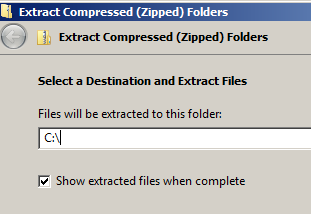
\includegraphics[width=0.3\textwidth]{images/esp/esp32win}
		\caption{Alamat Extrak Kompiler ESP32}
	\end{figure}
	
	Jika sukses akan tersedia folder \textbf{C:\textbackslash msys32}.
	Kemudian jalankan terminal \textbf{C:\textbackslash msys32\textbackslash mingw32.exe}
	
	\newpage
	\begin{figure}[!ht]
		\centering
		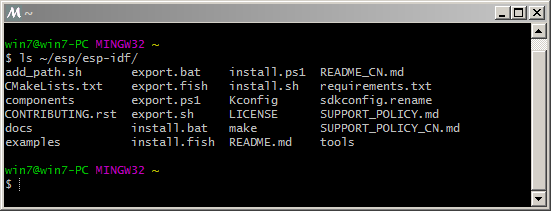
\includegraphics[width=0.6\textwidth]{images/esp/esp32mingw}
		\caption{Jendela Mingw ESP}
	\end{figure}
	
	instalasi dapat dicek dengan perintah di jendela tersebut
	\begin{minted}[frame=lines,framesep=2mm,fontsize=\normalsize,bgcolor=LightGray]{sh}
xtensa-esp32-elf-gcc --version
	\end{minted}
	
	\begin{figure}[!ht]
		\centering
		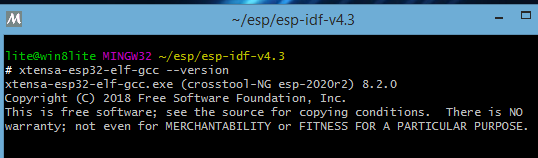
\includegraphics[width=0.6\textwidth]{images/esp/esp32ver}
		\caption{Version ESP32}
	\end{figure}
	
	\section{Instalasi Driver}
	
	Jika menggunakan board ESP32-DevKit, maka driver yang dibutuhkan adalah driver chip CP210x.
	Dapat didownload di: \url{https://www.silabs.com/developers/usb-to-uart-bridge-vcp-drivers}
	
	\section{Library ESP-IDF}
	
	\subsection{ArchLinux/Manjaro}
	
	Install versi 4.3 menggunakan PKGBUILD berikut: \href{https://github.com/mekatronik-achmadi/archlinuxmate/blob/main/pkgbuilds/optional/esp32-idf/PKGBUILD}{PKGBUILD}
	
	Atau versi terbaru dari: \url{https://aur.archlinux.org/packages/esp-idf}
	
	Kemudian untuk modul pustaka yang ditulis dengan Python, install Python versi 3.9 dari: \url{https://aur.archlinux.org/packages/python39}
	
	Selanjutnya, dibuat Python environment dengan perintah:
	
	\begin{minted}[frame=lines,framesep=2mm,fontsize=\normalsize,bgcolor=LightGray]{sh}
cd $HOME
virtualenv --python=/usr/bin/python3.9 esp32 --system-site-packages

source $HOME/esp32/bin/activate
pip install kconfiglib future cryptography pyserial pyparsing==2.2.0
deactivate
	\end{minted}
	
	\subsection{Windows}
	
	Pertama, jalankan kembali terminal \textbf{C:\textbackslash msys32\textbackslash mingw32.exe}.
	
	Kemudian buat folder dengan perintah:
	
	\begin{minted}[frame=lines,framesep=2mm,fontsize=\normalsize,bgcolor=LightGray]{sh}
mkdir -p ~/esp/;cd ~/esp/
	\end{minted}
	
	Unduh versi 4.3 di alamat: \url{https://dl.espressif.com/dl/esp-idf/releases/esp-idf-v4.3.zip}
	
	Ekstrak ke alamat \textbf{C:\textbackslash msys32\textbackslash home\textbackslash username\textbackslash esp}.
	Dapat dicek hasil ekstrak dengan perintah:
	
	\begin{minted}[frame=lines,framesep=2mm,fontsize=\normalsize,bgcolor=LightGray]{sh}
ls ~/esp/esp-idf-v4.3/
	\end{minted}
	
	Selanjutnya, update submodule dengan perintah:
	
	\begin{minted}[frame=lines,framesep=2mm,fontsize=\normalsize,bgcolor=LightGray]{sh}
cd ~/esp/esp-idf-v4.3/
git submodule update --init
	\end{minted}
	
	Definisikan alamat \textbf{IDF\_PATH}:
	
	\begin{minted}[frame=lines,framesep=2mm,fontsize=\normalsize,bgcolor=LightGray]{sh}
export IDF_PATH=$HOME/esp/esp-idf-v4.3
	\end{minted}
	
	Selanjutnya, update kebutuhan Python:
	
	\begin{minted}[frame=lines,framesep=2mm,fontsize=\normalsize,bgcolor=LightGray]{sh}
python3 -m pip install --user -r $IDF_PATH/requirements.txt
	\end{minted}
	
	%%%%%%%%%%%%%%%%%%%%%%%%%%%%%%%%%%%%%%%%%%%%%%%%%%%%%%%%%%%%%%%%%
	
	\chapter{Text Editor}
	
	Beberapa text editor programming yang direkomendasikan
	
	\section{Geany}
	
	Geany adalah teks editor ringan berbasis GTK3.
	Dapat diinstall dengan:
	
	\begin{itemize}
		\item ArchLinux/Manjaro
		\begin{minted}[frame=lines,framesep=2mm,fontsize=\normalsize,bgcolor=LightGray]{sh}
sudo pacman -S geany geany-plugins
		\end{minted}
		
		\item MSYS2
		\begin{minted}[frame=lines,framesep=2mm,fontsize=\normalsize,bgcolor=LightGray]{sh}
pacman -S mingw-w64-x86_64-geany mingw-w64-x86_64-geany-plugins
		\end{minted}
		
		\item Windows. Installer dan plugin tersedia di:
		\url{https://www.geany.org/download/releases/}
	\end{itemize}
	
	\begin{figure}[!ht]
		\centering
		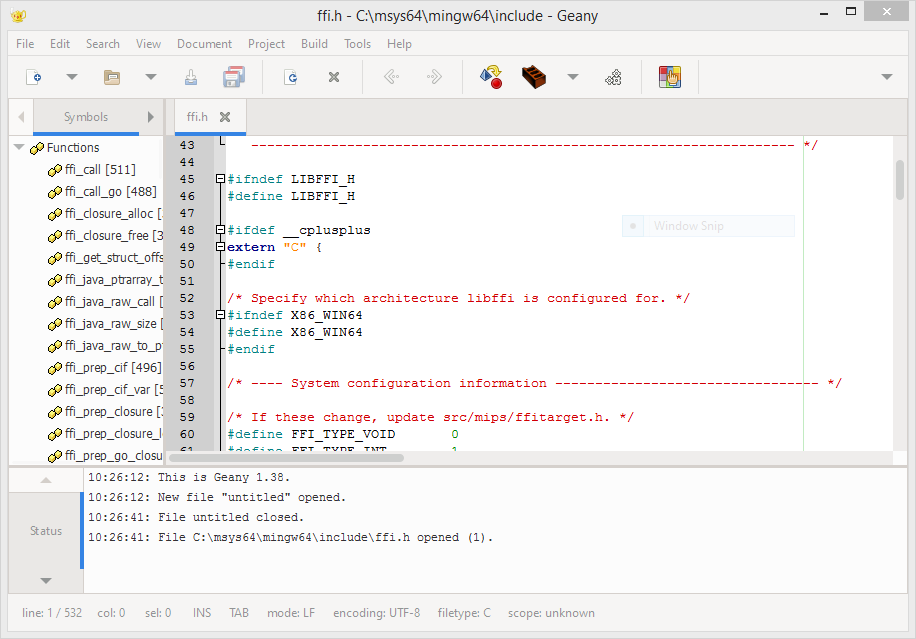
\includegraphics[width=0.65\textwidth]{images/editor/geany}
		\caption{Geany}
	\end{figure}
	
	\newpage
	\section{VSCodium}
	
	Visual Studio Code adalah editor extensible berbasis framework Electron dari Microsoft.
	VSCodium merupakan varian open-source dengan fitur Microsoft dikurangi.
	Dapat diinstall dengan:
	
	\begin{itemize}
		\item ArchLinux/Manjaro. \url{https://aur.archlinux.org/packages/vscodium-bin}
		\item Windows. \url{https://github.com/VSCodium/vscodium/releases}
	\end{itemize}
	
	\begin{figure}[!ht]
		\centering
		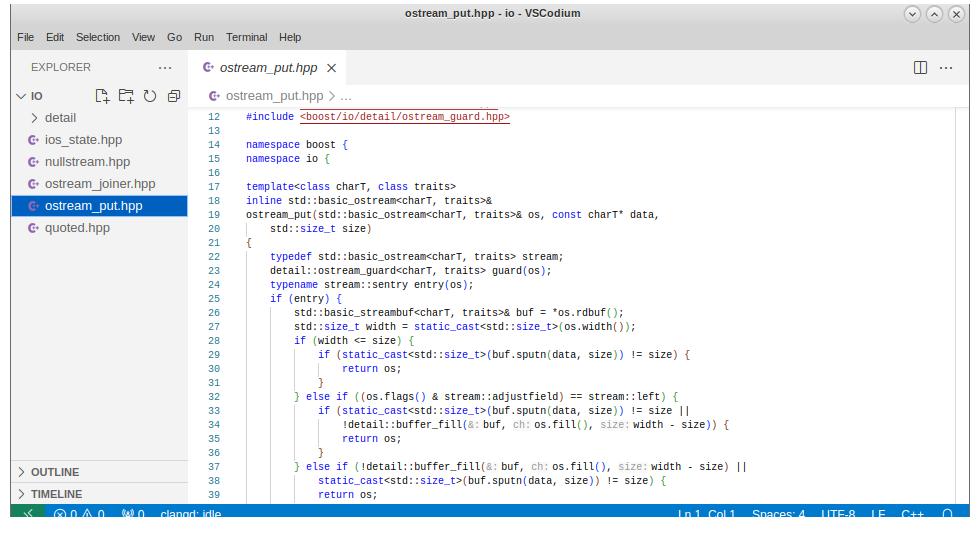
\includegraphics[width=0.7\textwidth]{images/editor/vscodium}
		\caption{VSCodium}
	\end{figure}
	
	Beberapa ekstensi yang direkomendasikan:
	
	\begin{itemize}
		\item Clangd. \url{https://github.com/clangd/vscode-clangd/}
		\item Doxygen. \url{https://github.com/cschlosser/doxdocgen/}
	\end{itemize}
	
	%%%%%%%%%%%%%%%%%%%%%%%%%%%%%%%%%%%%%%%%%%%%%%%%%%%%%%%%%%%%%%%%%
	
\end{document}
